% Drawing 86/01-10 -- folder 86, batch 01, archive page 7 (PDF page 8).
% Transcription: en bas à droite, à l'encre épaisse sur un tracé au crayon : un icosaèdre vu de face sur une arête, ses douze sommets visibles, une arête cachée horizontale en tirets ; au-dessus, un petit croquis de trois cercles qui se recoupent autour d'un petit polyèdre.
% Kind: icosahedron seen edge-on (ink over pencil); three overlapping circles round a small polyhedron. Method 2 (schematic redraw from the facsimile). Status: partial.
% Notes: Large figure: the twelve vertices as read and the 27 inked edges that can be followed between them (outline: top, two upper corners, two lower corners, bottom; inside: the upper centre on the top horizontal, a horizontal edge between two middle vertices with a vertical edge under each, the lower centre and the edges to it), and the dashed horizontal between the two lower corners. Small sketch above: three circles overlapping two by two and, where they meet, a small hexagonal outline with a triangle inside it. Left out: the pencil underdrawing round the large figure (a looser outline and a frame, which the transcription reads as a cube), several short dashed strokes inside it, and the inner strokes of the small polyhedron. Still differs: the edge list of the large figure is what the ink shows, not a checked icosahedron (27 solid edges and one dashed are drawn; the page may hold two or three more under the heavy ink); the small sketch is schematic. Decided by a machine pass, 2026-11-12: the heavy figure is recorded as an icosahedron seen along an axis through the middle of an edge, the pencil frame round it not being legible as a cube with its edges. Not checked by a reader. Redrawn 2026-11-12 (issue 128): to check again.
% Coordinates: 1 unit = 1 mm = 1/100 of the crop width (bbox in page fractions: [0.62, 0.56, 0.94, 0.88]).
% Redrawn by Claude (claude-fable-5-2), issue #128, 2026-11-12; not checked by a human; not compiled (no TeX in the session).
% Rights: reproduces part of the work -- behind RENDER_TRANSCRIPTS, never published by itself.
\documentclass[tikz,border=3pt]{standalone}
\usepackage{amsmath,amssymb}
\usetikzlibrary{patterns,arrows.meta}
\tikzset{pencil/.style={black!45}, struck/.style={black!35}, mpt/.style={circle,draw,inner sep=1.3pt}, pt/.style={circle,fill,inner sep=0.9pt}, opt/.style={circle,draw,fill=white,inner sep=1.1pt}}
\begin{document}
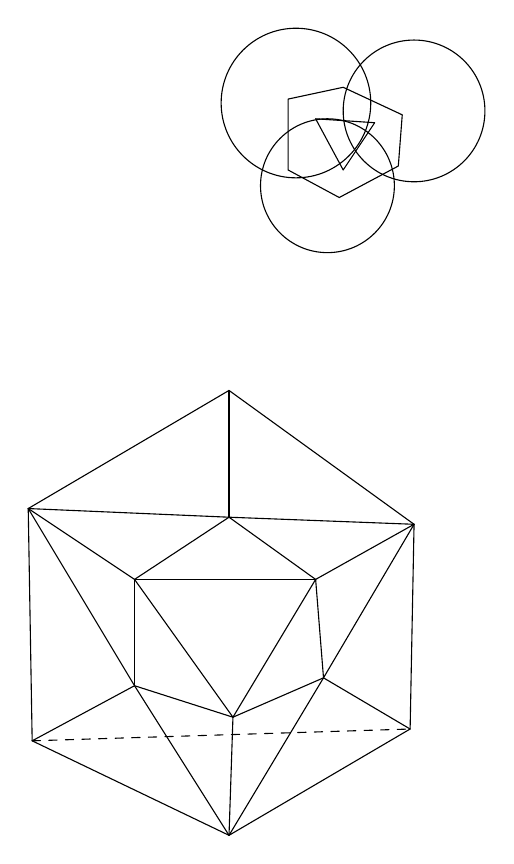
\begin{tikzpicture}[x=1mm,y=1mm,line cap=round,line join=round,font=\scriptsize]
\draw (42.5,-65.5) -- (17,-80.5);
\draw (42.5,-65.5) -- (66,-82.5);
\draw (42.5,-65.5) -- (42.5,-81.6);
\draw (17,-80.5) -- (42.5,-81.6);
\draw (42.5,-81.6) -- (66,-82.5);
\draw (42.5,-81.6) -- (30.5,-89.5);
\draw (42.5,-81.6) -- (53.5,-89.5);
\draw (17,-80.5) -- (30.5,-89.5);
\draw (66,-82.5) -- (53.5,-89.5);
\draw (30.5,-89.5) -- (53.5,-89.5);
\draw (17,-80.5) -- (17.5,-110);
\draw (66,-82.5) -- (65.5,-108.5);
\draw (30.5,-89.5) -- (30.5,-103);
\draw (53.5,-89.5) -- (54.5,-102);
\draw (17,-80.5) -- (30.5,-103);
\draw (66,-82.5) -- (54.5,-102);
\draw (30.5,-89.5) -- (43,-107);
\draw (53.5,-89.5) -- (43,-107);
\draw (30.5,-103) -- (43,-107);
\draw (54.5,-102) -- (43,-107);
\draw (17.5,-110) -- (30.5,-103);
\draw (65.5,-108.5) -- (54.5,-102);
\draw (17.5,-110) -- (42.5,-122);
\draw (65.5,-108.5) -- (42.5,-122);
\draw (43,-107) -- (42.5,-122);
\draw (30.5,-103) -- (42.5,-122);
\draw (54.5,-102) -- (42.5,-122);
\draw[dashed] (17.5,-110) -- (65.5,-108.5);
\draw (51,-29) circle[radius=9.5];
\draw (66,-30) circle[radius=9];
\draw (55,-39.5) circle[radius=8.5];
\draw (57,-27) -- (64.5,-30.5) -- (64,-37) -- (56.5,-41) -- (50,-37.5) -- (50,-28.5) -- cycle;
\draw (53.5,-31) -- (61,-31.5) -- (57,-37.5) -- cycle;
\end{tikzpicture}
\end{document}
